\documentclass[10pt]{article}
\usepackage[a4paper,margin=0.8in]{geometry}
\usepackage{booktabs}
\usepackage{graphicx}
\usepackage{enumitem}
\usepackage[hidelinks]{hyperref}
\setlist{topsep=2pt,itemsep=1pt,parsep=0pt}
\setlength{\parindent}{0pt}
\setlength{\parskip}{4pt}
\title{\vspace{-1.5em}Data Analytics 1, Assignment 2, Part 1:\\Snowflake Warehouse for a Brazilian Marketplace}
\author{}
\date{}
\begin{document}
\maketitle
\vspace{-3em}

\section*{1. Schema}
The warehouse is a Snowflake schema in DuckDB, with real primary and foreign keys.
\textbf{Grain of the fact table: one row per item line of an order} (\texttt{order\_id} + \texttt{order\_item\_id}); \texttt{fact\_order\_item} has 112,650 rows.
A second fact, \texttt{fact\_order\_payment}, has one row per payment (103,886 rows). It stays separate because payments belong to orders, not items, so joining them to items would multiply revenue.

\textbf{Hierarchies normalised, and why:}
\begin{itemize}
\item \textbf{Geography:} zip $\to$ city $\to$ state $\to$ region. Customers and sellers both point to this one hierarchy, so ``Southeast'' means the same thing for both. Region is not in the data; it comes from a seed file of the 27 states and the five official regions.
\item \textbf{Product:} product $\to$ category, with the English name stored once per category.
\item \textbf{Seller:} seller $\to$ acquisition $\to$ lead origin, with business segment and won date on the acquisition level.
\item \textbf{Calendar:} date $\to$ month $\to$ quarter $\to$ year, which supports the time roll-ups directly.
\end{itemize}
\texttt{dim\_order} holds all 99,441 orders, and \texttt{dim\_review} holds every review row, because an order can have several reviews and one \texttt{review\_id} can cover several orders. Key $-1$ is the Unknown member of a dimension, so a missing value never drops a row. The ER diagram is in \texttt{diagrams/er\_diagram.png} and on the last page.

\section*{2. ETL}
\begin{enumerate}
\item \textbf{Staging:} each CSV lands unchanged as text in a \texttt{stg} table.
\item \textbf{Dimensions, top-down:} region, state, city, zip, then the tables that depend on them. The foreign keys reject any other order, so top-down loading is enforced, not just followed.
\item \textbf{Facts:} loaded last, with \texttt{revenue = price + freight\_value} as an exact decimal.
\item \textbf{Validation:} 24 checks; the ETL fails if any is wrong. All 24 pass.
\end{enumerate}
\textbf{Data problems found and handled:}
\begin{itemize}
\item \textbf{Zips with several cities.} 8,556 zip prefixes appear with more than one city spelling or city. City names were normalised (case, accents, apostrophes), then the most frequent state and city per zip were chosen, with ties broken alphabetically. This gives a strict hierarchy. Only 181 customers (0.18\%) end up with a city different from the one they typed.
\item \textbf{Zips missing from the geolocation file:} 157 customer and 7 seller prefixes fall back to the cleaned address text, which removes entries such as ``sao paulo - sp''.
\item \textbf{Wrong seller states.} 35 sellers typed a state that contradicts their own zip and city, for example Curitiba marked SP. The zip hierarchy corrects them, which is why Q7 shows 22 seller states, not the 23 in the raw file.
\item \textbf{Categories:} 610 products have no category and go to Unknown. Two categories had no English name and were added in a seed file.
\item \textbf{Orders kept:} 768 orders with no review, 2,965 with no delivery date and 775 with no items all stay in \texttt{dim\_order}.
\item \textbf{Funnel:} only 380 of the 842 closed deals match a seller in \texttt{sellers.csv}. All 842 stay in the acquisition table; the 2,715 sellers with no deal are labelled \texttt{not\_in\_funnel}.
\end{itemize}

\section*{3. Insights}
Revenue is \textbf{R\$ 15,843,553.24} across 98,666 orders, with revenue counted on the purchase date. It includes every item regardless of status; delivered orders are 97.33\% of it.

\textbf{Q1--Q2, time.} Revenue grew from R\$ 7.14M in 2017 to R\$ 8.64M in 2018, but neither end of the range is a full period: 2016 holds only R\$ 57,183, and sales effectively stop in August 2018 (September has R\$ 166). Peak months were October 2016, November 2017 (R\$ 1.18M) and April 2018 (R\$ 1.16M). The best quarter was Q2 2018 (R\$ 3.33M).

\textbf{Q3--Q4, products.} The top three categories are health\_beauty (R\$ 1.44M, 9.1\%), watches\_gifts (8.24\%) and bed\_bath\_table (7.84\%). Seven categories make up about half of revenue. No single product dominates: the top health\_beauty product by units earns only 0.7\% of its category. The best seller overall sold 527 units, in furniture\_decor.

\textbf{Q5, geography.} On customer location, the Southeast earns \textbf{64.58\%} of revenue, São Paulo state 37.38\% and the city of São Paulo 13.7\%. Order value runs the other way: R\$ 223 per order in the North against R\$ 151 in the Southeast, which is consistent with freight being part of revenue.

\textbf{Q6, customers.} Grouping uses \texttt{customer\_unique\_id}, because \texttt{customer\_id} is issued per order: 99,441 ids belong to 96,096 people, and 2,997 of them bought more than once. The top customer spent R\$ 13,664.08 in one order of 8 items in Rio de Janeiro. The second, at R\$ 7,571.63, placed 2 orders and would be split apart by \texttt{customer\_id}.

\textbf{Q7, sellers.} São Paulo has 1,816 sellers and its leader takes only 2.46\% of state revenue. Smaller states depend on very few sellers: one seller holds 76.88\% of Bahia. This is a concentration risk for the marketplace. States with one seller show 100\% by construction.

\textbf{Q8, cube.} \texttt{CUBE(region, category, year)} gives 8 group-bys and 1,342 rows, with 718 cells at the finest level. Each of the 8 slices re-sums to R\$ 15,843,553.24, so revenue is fully additive. The largest region--category pair is Southeast bed\_bath\_table (R\$ 921,076). Leaders differ by region: bed\_bath\_table in the Southeast, sports\_leisure in the South, and health\_beauty in the other three.

\textbf{Q9, delivery and reviews.} This runs at order grain, so an order with many items counts once. ``Late'' compares the delivered date with the estimated date.
\begin{center}\small
\begin{tabular}{lrrr}
\toprule
Delivery & Orders & Average review & Scores of 1--2 \\
\midrule
Early & 88,644 & 4.294 & 9.2\% \\
On time & 1,292 & 4.036 & 12.3\% \\
Late, 1--7 days & 3,672 & 2.715 & 49.4\% \\
Late, over 7 days & 2,862 & 1.698 & 79.2\% \\
\emph{All late} & 6,534 & 2.272 & 62.4\% \\
Not delivered & 2,971 & 1.754 & 77.7\% \\
\bottomrule
\end{tabular}
\end{center}
Orders delivered more than a week late average 1.70, against 4.04 for on-time orders. This is a strong association, not proof of cause: late orders may also differ in product, seller or region, and a controlled test would be needed to measure the effect. Grain matters too: at item grain the early average falls to 4.212, because large orders are counted once per item.

\textbf{Q10, marketing channel.} Among sellers with a known source, \texttt{organic\_search} leads the named channels with R\$ 235,957 (30.41\% of funnel revenue), ahead of \texttt{paid\_search} (23.46\%). The label \texttt{unknown} is slightly larger, at R\$ 240,161. The main caution is coverage: \textbf{sellers with an origin earn only 4.9\% of revenue}, because the funnel data covers only recent recruits. The ranking describes that group, not the marketplace.

\textbf{Reconciliation.} Payments total R\$ 16,008,872.12, which is R\$ 165,318.88 more than item revenue. The gap is fully explained:
\begin{center}\small
\begin{tabular}{lrr}
\toprule
Orders & Count & Gap (R\$) \\
\midrule
Payment but no items & 775 & 162,591.95 \\
Paid more than item revenue & 241 & 3,069.65 \\
Paid less than item revenue & 19 & $-$198.63 \\
Items but no payment & 1 & $-$143.46 \\
Match within 5 centavos (rounding) & 98,405 & $-$0.63 \\
\midrule
Total & 99,441 & 165,318.88 \\
\bottomrule
\end{tabular}
\end{center}
235 of the 241 overpaid orders used instalments, which suggests instalment interest, although the data does not state it.

\clearpage
\section*{Appendix: ER diagram}
\begin{center}
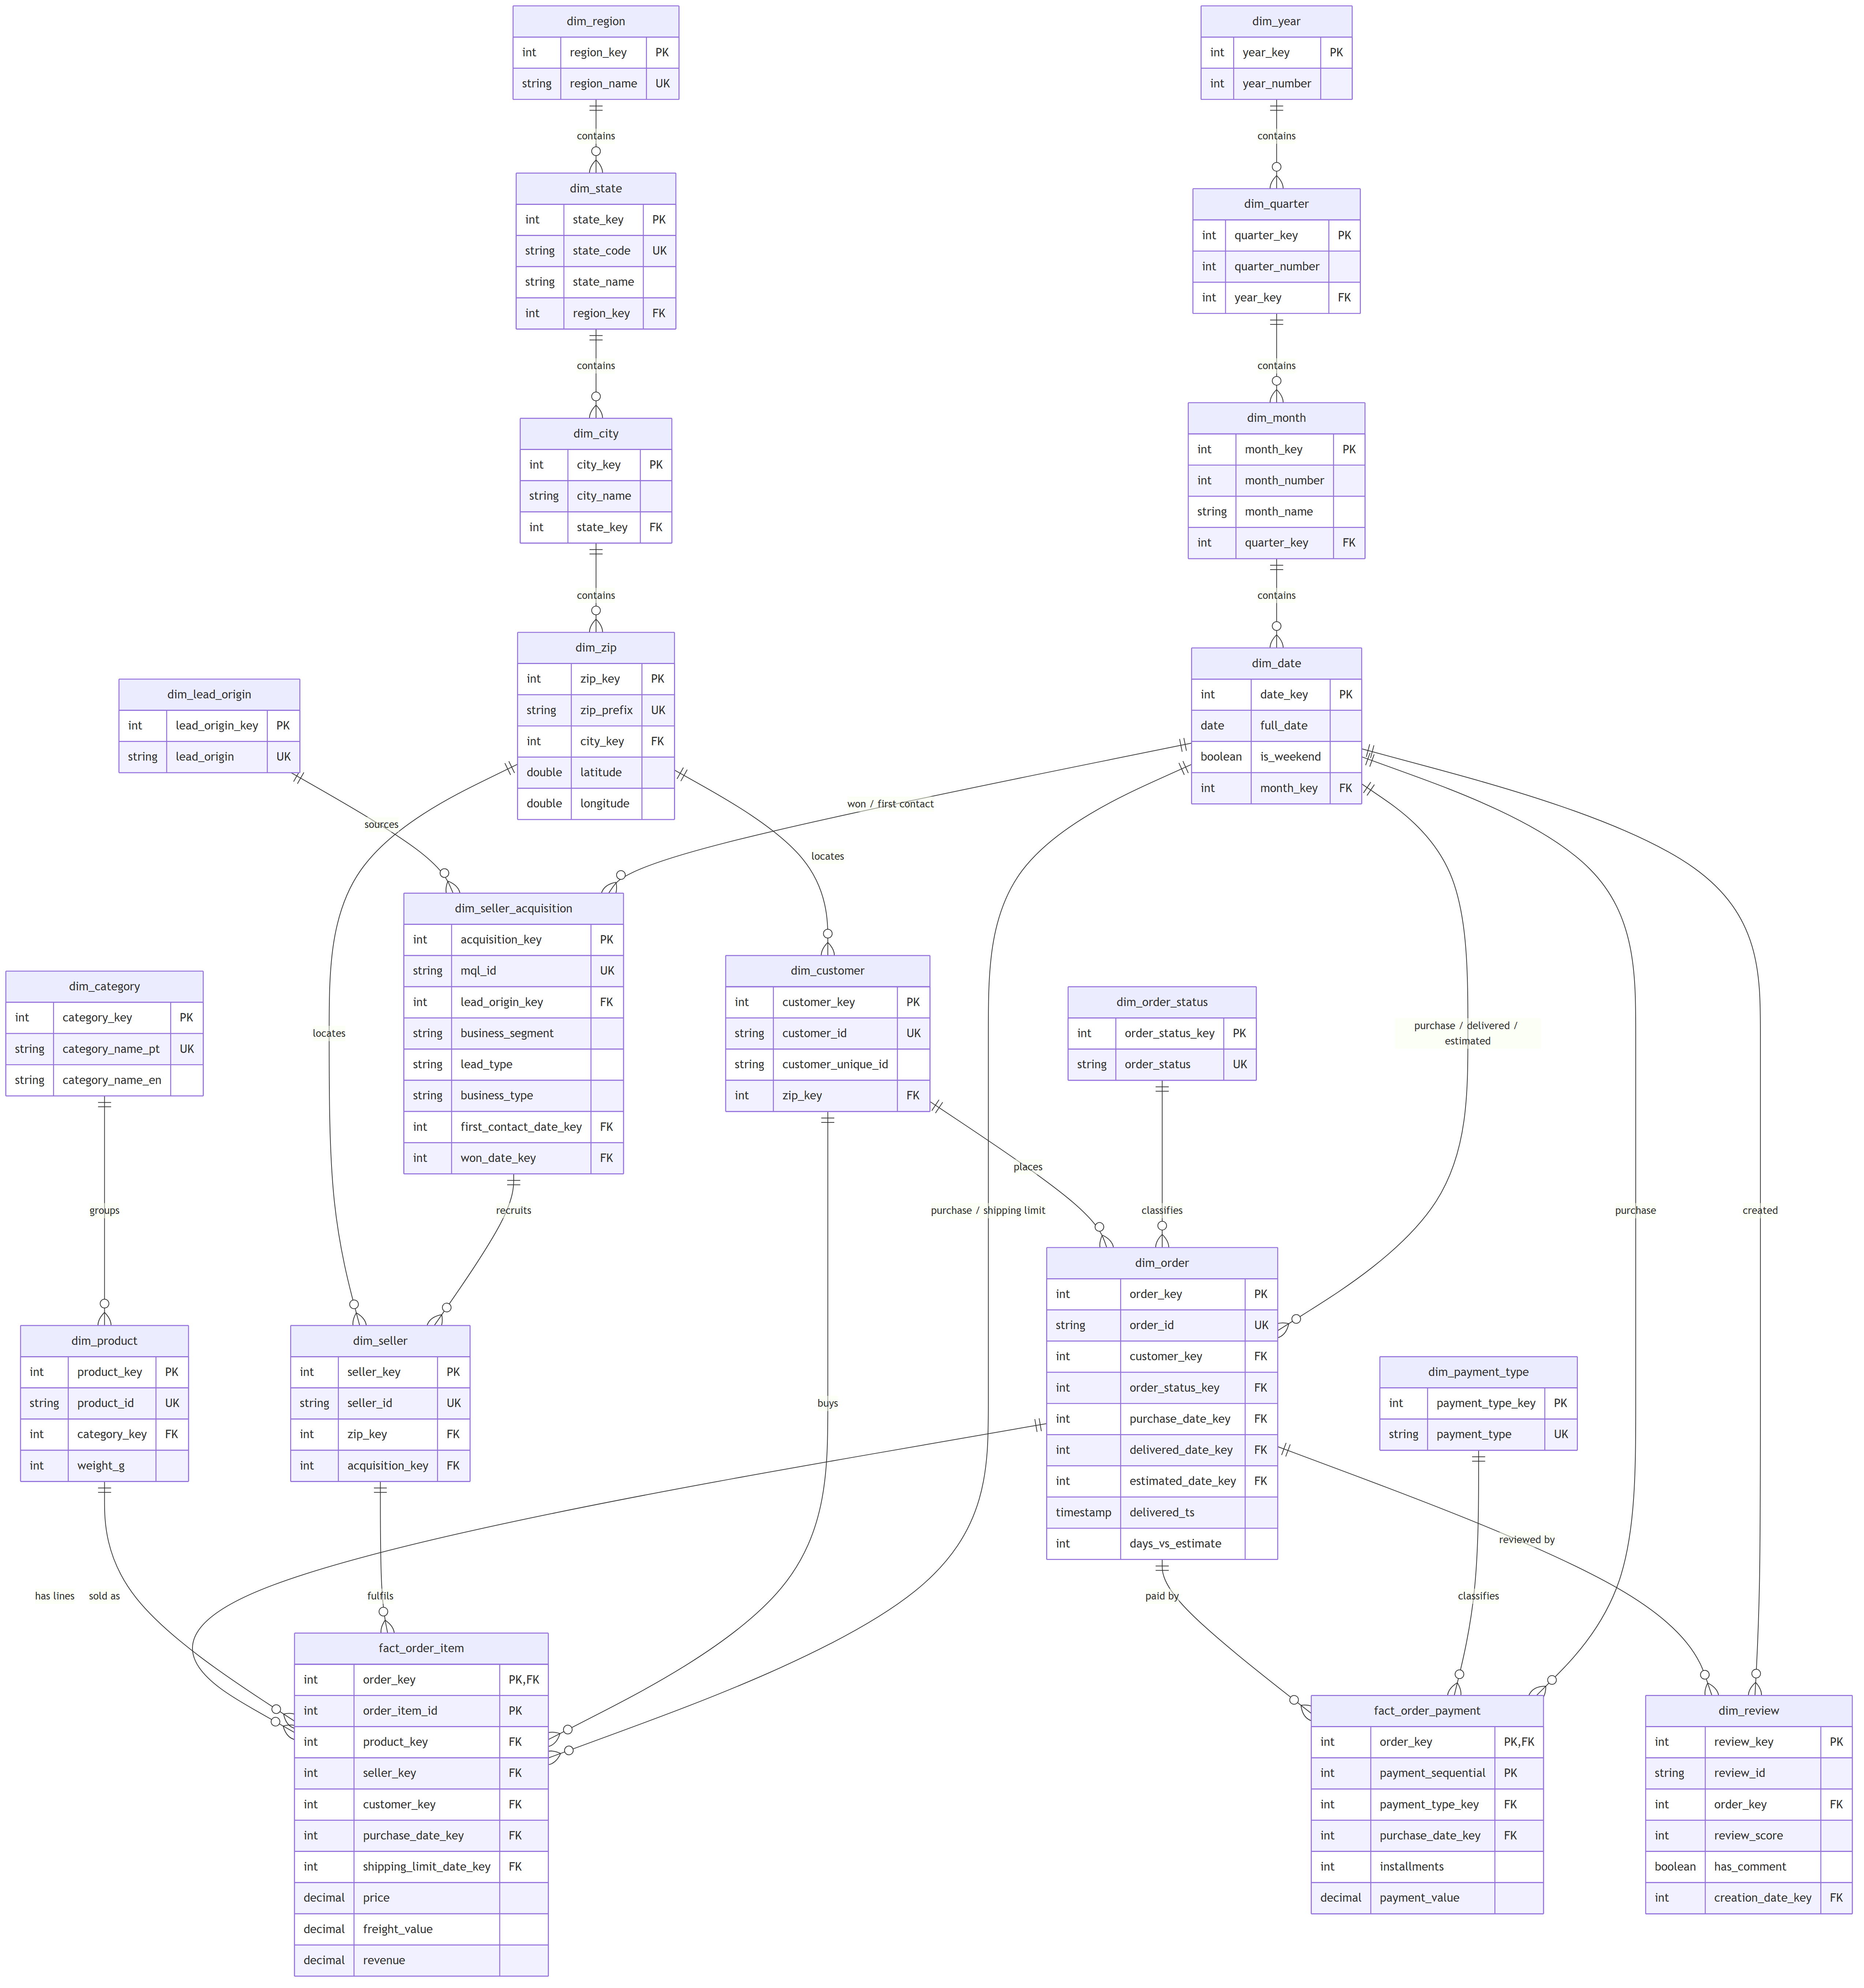
\includegraphics[width=\textwidth,height=0.9\textheight,keepaspectratio]{../diagrams/er_diagram.png}
\end{center}
\end{document}
